\section{Methods} \label{sec:methods}

In this section, we detail the methodology for benchmark and validation experiments used to assess the performance of the proposed shortcut-enabled algorithm.

\subsection{Generation of Benchmark Data}

Across our benchmark experiments, we needed a large-scale sample of genomes to perform reconstructions on.
For this purpose, we performed simulations using the Cerebras CS-2
Wafer-Scale Engine, an 850,000 core hardware accelerator device \citep{lie2023cerebras}.
Processor elements (PEs) in this architecture are arranged in a grid lattice, with each processor able to execute independently and communicate with neighboring PEs through message-passing.

To conduct these simulations, we used an extension of the island-model genetic algorithm framework presented in \citep{moreno2024trackable}.
This framework organizes simulated organisms into independent subpopulations hosted on each PE.
Synchronous tournament selection of size 2 is applied within each PE, and between generations agents are migrated between PEs asynchronously.

%The purpose of this simulation was to generate large-scale data using a simple model that can be explicitly manipulated to explore evolutionary regimes differing substantially in the depth of shared ancestry between organisms (known as phylogenetic richness).

A simple genome model was used, comprised of a single floating point value representing fitness.
Reproduction occurred asexually, with this value subject to a normally-distributed mutation with 30\% probability.
(In the case of the purifying-regime treatment, the negative absolute value of a sampled mutation delta was applied.)
In tournament competitions to select parents for the subsequent generation, the parent was selected according to the higher fitness value with 10\% probability and was otherwise selected randomly.
Genomes were augmented with hstrat annotations comprising 64 single-bit markers, managed at runtime using a \texttt{tilted} curation policy, which favors dense retention of more recent marker data \citep{moreno2024structured}.

To generate data representative of differing evolutionary conditions, two treatments were applied: an
\textbf{adaptive regime} and a \textbf{purifying regime}.
Under the adaptive regime, mutations increasing fitness were allowed, introducing the possibility of selective sweeps.
By contrast, the purifying regime treatment allowed only deleterious mutations.
Previous work with this system demonstrated the purifying regime to exhibit substantially greater phylogenetic richness, in line with expectation for selective sweeps to diminish population-level phylogenetic diversity \citep{moreno2024trackable}.

% https://github.com/mmore500/wse-async-ga/blob/31034c3b1f8127763807992916f20d7d3ea62919/slurm/2024-12-25/2024-12-25%2Blex12-async-ga.sh
The simulation was run for 5 million generation cycles.
A per-PE population size of 256 organisms was used, providing a net population size of 190.8 million organisms.
% https://osf.io/btg23 and https://osf.io/2my97
``Fossil'' genome data was sampled on a rolling basis over the course of simulation using asynchronous \texttt{memcopy} operations, where sample genomes were copied from each PE on a rolling basis.
In total, collection of 1,999 (purifying regime) and 2,014 (adaptive regime) \texttt{memcopy} cycles elapsed.
% https://osf.io/btg23 and https://osf.io/2my97
Real-time runtime under each treatment was 24 minutes.

For implementation-level details on the Wafer-Scale Engine simulation, see \citep{moreno2024trackable}.

\subsection{Microbenchmark Experiments}

In a first set of microbenchmark trials, we performed a head-to-head comparison of the proposed shortcut-enabled algorithm with the previous naive trie-building approach.
Given performance limitations of the naive approach, the maximum reconstruction workload tested was limited to 10,000 genomes.
Experiments used random subsamples of genomes from WSE fossil data described above.
To facilitate informative comparison, timings measured just the trie-building component of reconstructions, excluding pre- and post-processing steps.
Five replicate observations were taken per timing.

In a second set of microbenchmark trials, we conducted an empirical scaling analysis of the shortcut-enabled trie building algorithm across a wider spread of reconstruction workload sizes.
To assess the relationship between marginal throughput and trie size, we performed trie reconstructions of 10 million WSE genomes, broken into successive batches of 100,000 genomes.
This approach allowed us to independently measure time taken to insert each batch, with the goal determining how this time changes for later batches (i.e., larger trees).
We also performed unbatched tests evaluating net execution time to build tries ranging from 1 to 10 million tips.
For these experiments, 3 replicates were performed per observation.

All microbenchmarks were replicated using genomes generated under adaptive and purifying regimes to assess sensitivity of performance to underlying phylogeny structure.

\subsection{Macrobenchmark Experiments}

To assess the performance of our approach on large-scale workloads under real-world conditions, we supplemented microbenchmarks focusing on core trie extension and consolidation operations with two macrobenchmark trials comprising the full end-to-end reconstruction pipeline described in Section \ref{sec:pipeline}.
To reduce peak memory use, we additionally included a step to collapse unnecessary unifurcations (i.e., parent nodes with only a single child) between trie-building batches --- for more details, see the supplemental \citep{supplemental}.
These end-to-end experiments used the \texttt{hstrat.dataframe.surface\_build\_tree} CLI module incorporated in the \texttt{hstrat} library.

These experiments were conducted using the full billion-genome corpus of fossil data gathered from Wafer-Scale Engine simulations.
We performed two trial reconstructions: one using genome data from the adaptive regime treatment and another under the purifying regime treatment.
Reconstructions were conducted on 100-core cluster node allocations with 2 TB of memory.

\subsection{Validation Tests}

By design, our proposed shortcut-enabled algorithm produces equivalent reconstruction results compared to the reference naive approach, up to arbitrary tie-breaking decisions (see supplemental material \citep{supplemental} for detailed discussion).
To confirm correctness of our implementation, however, we report several validation tests.%
\footnote{In addition to validation experiments reported here, note that the \texttt{hstrat} library includes an extensive unit tests that compare reconstructed most-recent common ancestor (MRCA) between organisms to the value expected by direct comparison of their hstrat marker records.}

% https://github.com/mmore500/hstrat/blob/277ea0ee4d6e0bb6d259538b5fa7b62fe9085b10/examples/evolve_dstream_surf.py
Validation tests employed small evolutionary simulations run locally, to allow collection of ground-truth data via \texttt{phylotrackpy} \citep{dolson2024phylotrack}.
Simulations propagated populations of 100 agents under neutral evolution conditions, with runs lasting 500 generations.
We configured these simulations to consider both synchronous and asynchronous generations.
Reconstructions over end-state genomes were tested, as well as reconstructions incorporating fossil genomes sampled at 50 generation intervals.
To assess reconstruction quality, we calculated error as triplet distance between the ground truth and reconstructed phylogenies \citep{critchlow1996triples}.

\subsection{End-to-end Reconstruction Implementation}
\label{sec:pipeline}

\begin{figure*}
% graphic source https://docs.google.com/presentation/d/1CKU1Rtz8Vbk-Std3zFmzBcACf7EBj3amTTOAGKdBluQ
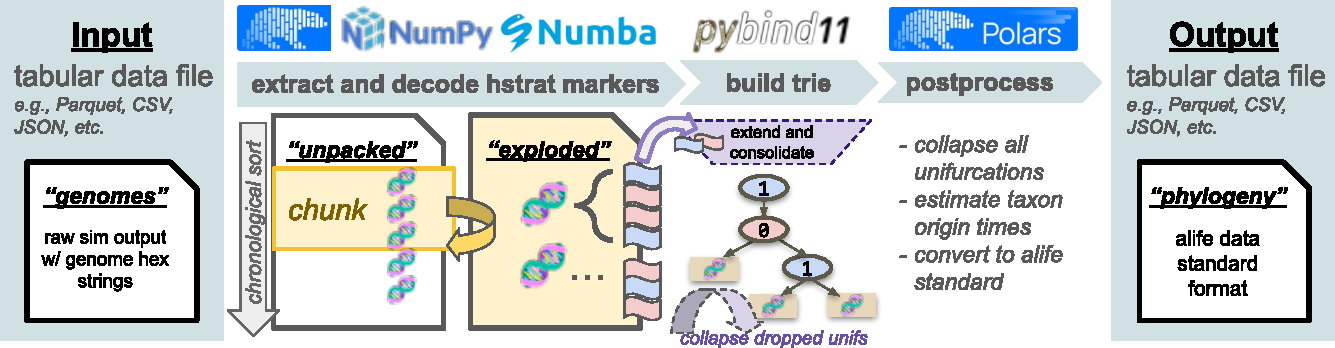
\includegraphics[width=\linewidth]{img/hstratpipeline.pdf}
\caption{\textbf{Schematic of hstrat phylogeny reconstruction pipeline.} TODO.}
\label{fig:hstratpipeline}
\end{figure*}


Figure \ref{fig:hstratpipeline} overviews the full end-to-end pipeline used to create a phylogenetic reconstruction from raw hstrat-annotated genome data.
First, hstrat annotation data is extracted and decoded.
To take advantage of SIMD parallelism, the decoding of origin times for genome markers is performed using bulk operations orchestrated via NumPy, batched over available processors using the Numba library threading engine.
Due to memory-intensity of the exploded representation, where each genome marker constitutes an individual dataframe row, a chunk size may be configured to limit the amount of data exploded at any one time.
A chunk size of 50 million genomes was used for macrobenchmark trials.

Subsequently, decoded marker data is fed genome-by-genome into the trie-building backend.
To ensure full hardware utilization, execution of the core trie-building procedure --- which is single-threaded --- is performed concurrently with decode/explode work on the upcoming chunk.
Finally, a phylogeny is extracted from the end-state trie, converted to alife standard format, and saved to disk.
The Polars library is used for load/save and other pre-/post-processing operations, allowing some operations to be distributed over available processor cores by the underlying threading engine.

\subsection{Software, Data, and Materials} \label{sec:materials}

Software used in this work is available via GitHub, and archived via Zenodo.%
\footnote{\scriptsize Benchmarking and validation code (v1.0.1) is available on GitHub at \href{https://github.com/mmore500/hstrat-reconstruction-algo/tree/v1.0.1}{\texttt{mmore500/hstrat-reconstruction-algo}} \citep{matthew_andres_moreno_2025_16898918}, WSE kernel code (v2025.12.26) for Cerebras SDK v1.0.0 at \href{https://github.com/mmore500/wse-async-ga/tree/v2025.12.26}{\texttt{mmore500/wse-async-ga}} \citep{moreno_2025_16898904}, and hstrat library code (v1.20.10) at \href{https://github.com/mmore500/hstrat/tree/v1.20.10}{\texttt{mmore500/hstrat}} \citep{moreno_2025_16898849}.}
Data and supplementary material is hosted via the Open Science Framework at \href{https://osf.io/63ucz/?view_only=2e3ec335c016436494ad125b14ffc8cb}{\texttt{osf.io/63ucz}} \citep{supplemental,foster2017open}.
All accompanying materials are provided open-source under the MIT License.

Microbenchmarks experiments were conducted on a 2019 MacBook Pro (2.3GHz 8-Core Intel i9, 16GB RAM) using a benchmark script provided with supplemental material \citep{supplemental}.
Head-to-head trie-building comparisons were performed using Python implementations of both algorithms.
Empirical scaling analysis experiments used a C++ implementation of the shortcut-enabled trie-building algorithm.

Macrobenchmarks were performed on AMD EPYC compute cluster nodes with 128 cores and 2005 GB of memory.
Purifying- and adaptive-regime reconstructions were performed on separate nodes with EPYC 7763 (2.445 GHz) and EPYC 7H12 (2.595 GHz) processors, respectively.
% purifying log: https://osf.io/gj52m
% adaptive log: https://osf.io/s3rzj
% Adaptive-regime reconstruction was performed on an AMD EPYC 7H12 Processor (2.595 GHz) with 128 cores and 2005 GB of memory.
End-to-end experiments also used a C++ implementation of the shortcut-enabled trie-building algorithm.

This project benefited significantly from open-source scientific software \citep{2020SciPy-NMeth,harris2020array,reback2020pandas,mckinney2010data,waskom2021seaborn,hunter2007matplotlib,moreno2022hstrat,yang2025downstream}.
